\documentclass{article}
\usepackage{fancyhdr}
\usepackage[utf8]{inputenc}
\usepackage[english]{babel}
\usepackage{tikz, multicol, graphicx, etoolbox, enumerate, setspace, relsize, mathrsfs, verbatim}
\usepackage{amsmath, amsfonts, amssymb, amsthm, epsfig, epstopdf, titling, url, array, esvect, tikz-3dplot}
\usepackage{graphicx}
\usepackage{hyperref}

\usepackage{listings}
\usepackage{xcolor}

\definecolor{codegreen}{rgb}{0,0.6,0}
\definecolor{codegray}{rgb}{0.5,0.5,0.5}
\definecolor{codepurple}{rgb}{0.58,0,0.82}
\definecolor{backcolour}{rgb}{0.95,0.95,0.92}


\usepackage{pgfplots}
\usepackage{tcolorbox}
\usepackage{amsthm}
\usepackage{cancel}
\usepackage[left=1in,right=1in,top=1in,bottom=1in]{geometry}
\usepackage[tableaux]{prooftrees}

\lstdefinestyle{mystyle}{
    backgroundcolor=\color{backcolour},   
    commentstyle=\color{codegreen},
    keywordstyle=\color{magenta},
    numberstyle=\tiny\color{codegray},
    stringstyle=\color{codepurple},
    basicstyle=\ttfamily\footnotesize,
    breakatwhitespace=false,         
    breaklines=true,                 
    captionpos=b,                    
    keepspaces=true,                 
    numbers=left,                    
    numbersep=5pt,                  
    showspaces=false,                
    showstringspaces=false,
    showtabs=false,                  
    tabsize=2
}

\lstset{style=mystyle}

\pagestyle{fancy}
\fancyhf{}
\fancyhead[L,RO]{Tasksheet 3}
\fancyhead[R,RO]{Fundamentals of Computational Mathematics}
\fancyfoot[L,RO]{Xiang Gao}
\fancyfoot[R,RO]{Math 4610}
\renewcommand{\headrulewidth}{0.4pt}% Default \headrulewidth is 0.4pt
\renewcommand{\footrulewidth}{0.4pt}% Default \footrulewidth is 0pt
\def\checkmark{\tikz\fill[scale=0.4](0,.35) -- (.25,0) -- (1,.7) -- (.25,.15) -- cycle;} 

\begin{document}

\section*{Task 1}
I used the example from Tasksheet $02$, namely 
$$f''(x) \approx \dfrac{f(x+h) - 2f(x) + f(x+h)}{h^2}, \,\,\, f(x) = cos(x)$$
to print out the following table, 
\begin{center}
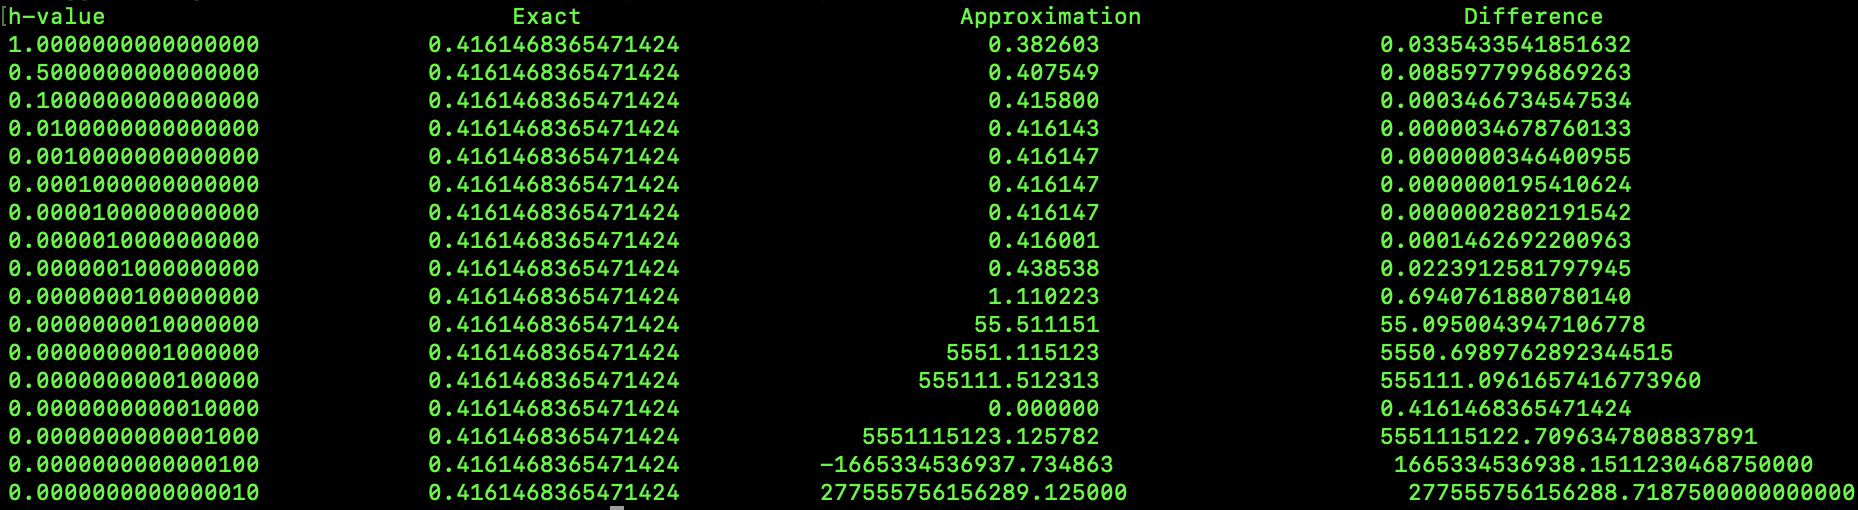
\includegraphics[width=\textwidth]{Screenshots/difference.png}
{\bf Figure 1.} Output Table.
\end{center}
And the following code is used:\\
\lstinputlisting[language=Python]{Task_1.py}

To verify if the central difference approximation is actually second order accurate. We can focus on the values associated with $h < 10^{-1}$.\\ 
The error decreases from $0.00034$, which suggests that the approximation is actually second order accurate.

\newpage

\section*{Task 2}
The central difference approximation is actually second order accurate due to the slope generated from the plot. \\
From the log-log plot, the approximation begins to fail around the $7$-th to $9$-th iteration. This is likely due to the limitation of python with decreasing $h$-value.
\begin{center}
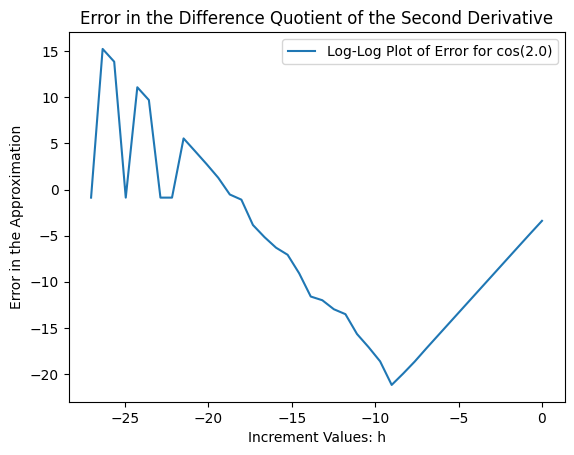
\includegraphics[width=7.5cm]{Screenshots/YourWay.png} \hspace{10pt} 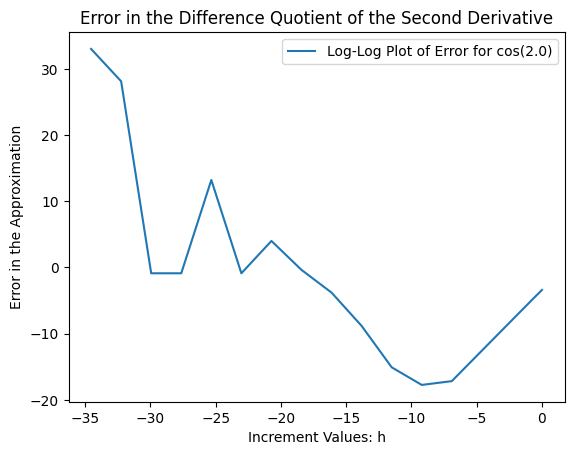
\includegraphics[width=7.5cm]{Screenshots/MyWay.png}\\
{\bf Figure 2.} Plot Generated Using Provided Code. \hspace{12pt} {\bf Figure 3.} Plot Generated Using Own Code. 
\end{center}
Since the I only changed two values in the provided code, my own code for {\bf Figure 3} is the following:
\lstinputlisting[language=Python]{Task_2Again.py}

\pagebreak

\section*{Task 3}
The routine for single precision is provided below:
\lstinputlisting[language=Python]{sMachineEps.py}
With the following code for testing:
\lstinputlisting[language=Python]{test_sMachineEps.py}
And the following output:
\begin{center}
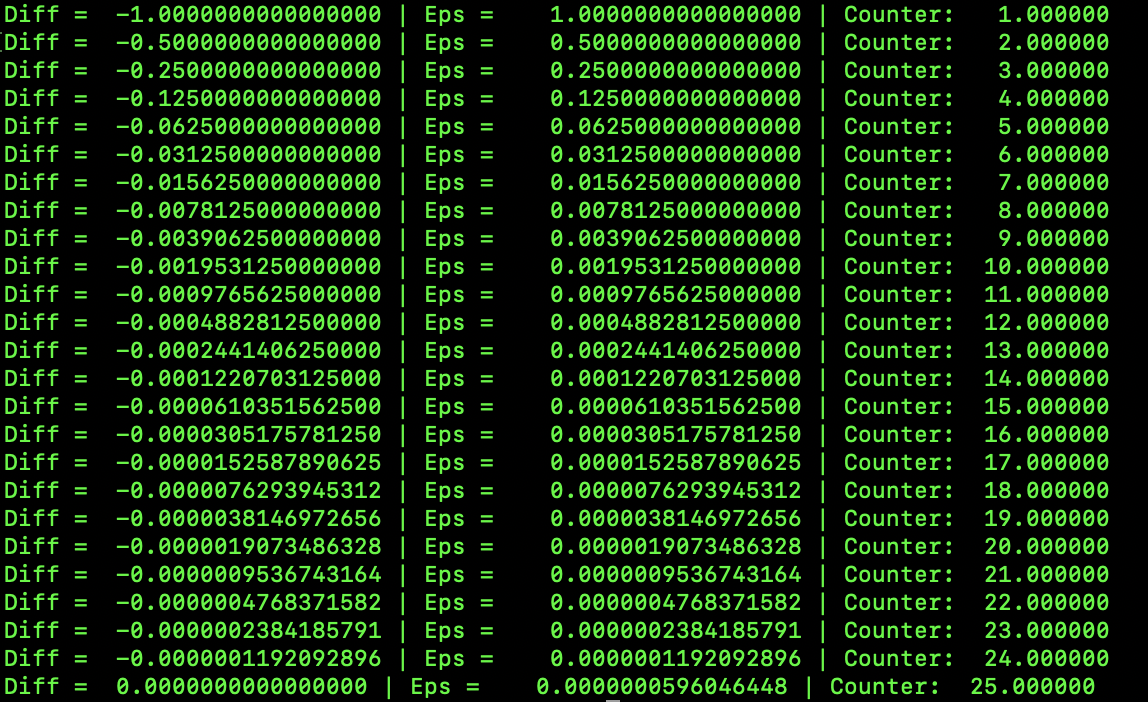
\includegraphics[width=\textwidth]{Screenshots/single.png}
{\bf Figure 4.} Machine Epsilon Single Precision Output:
\end{center}
The routine for double precision is provided below:
\lstinputlisting[language=Python]{dMachineEps.py}
With the following code for testing:
\lstinputlisting[language=Python]{test_dMachineEps.py}
And the following output:
\begin{center}
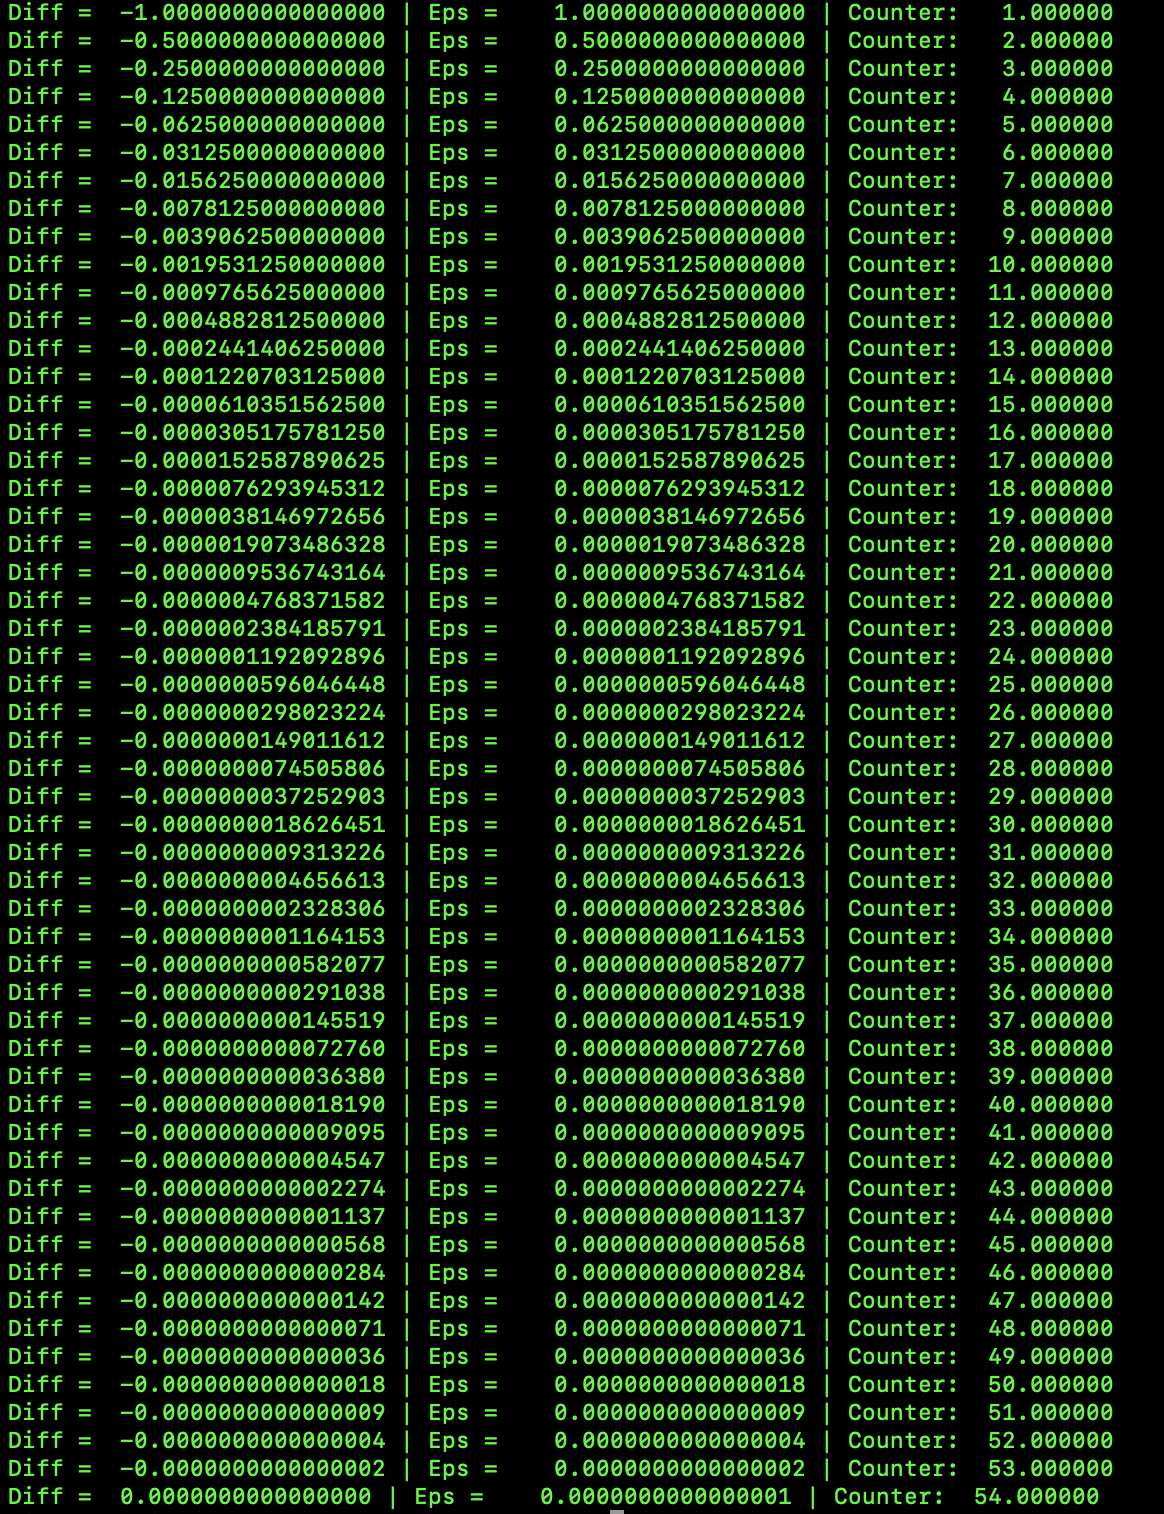
\includegraphics[scale = 0.74]{Screenshots/double.png}\\
{\bf Figure 5.} Machine Epsilon Double Precision Output.
\end{center}

\pagebreak

\section*{Task 4}
I created the \href{https://github.com/GoByMark/math4610/blob/fc8000ef7021a30b30a2c3733014ef5a0f7fed78/Homework_Tasks/Software_Manual/Software_Manual_toc.md}{Software Manual's Table of Contents}. Then I uploaded my precision calculating file. Afterward, I added the links to those files to the Software Manual's Table of Contents.

\vspace{5pt}

\section*{Task 5}
I have created and compiled and linked my shared library. It can be found \href{https://github.com/GoByMark/math4610/blob/d0507f36da5cdfa2d51124cb446eefca3e7cf3a4/Homework_Tasks/Tasksheet_03/src/mylib.a}{here}\

\vspace{5pt}

\section*{Task 6}
There are difference between static and \href{https://stackoverflow.com/questions/2649334/difference-between-static-and-shared-libraries}{shared libraries}\footnote{https://stackoverflow.com/questions/2649334/difference-between-static-and-shared-libraries}. 
	\begin{enumerate}
	\item Shared libraries reduce the amount of code that is duplicated in each program that makes use of the library, keeping the binaries small.
	\item Static libraries increase the overall size of the binary, but it means that you don't need to carry along a copy of the library that is being used.
	\end{enumerate}
There are also different kinds of \href{https://www.jenkins.io/doc/book/pipeline/shared-libraries/}{shared libraries}\footnote{https://www.jenkins.io/doc/book/pipeline/shared-libraries/}. For examples:
\begin{enumerate}
	\item Global Shared Libraries;
	\item Folder-level Shared Libraries;
	\item Automatic Shared Libraries
	\end{enumerate}

\end{document}